\documentclass[11pt,a4paper]{article}
\usepackage[utf8]{inputenc}
\usepackage[T1]{fontenc}
\usepackage{amsmath,amssymb}
\usepackage{booktabs}
\usepackage{geometry}
\usepackage{enumitem}
\usepackage{xcolor}
\usepackage{hyperref}
\usepackage{tikz}
\usetikzlibrary{arrows.meta,positioning}
\geometry{margin=2.4cm}
\definecolor{accent}{RGB}{38,70,83}
\hypersetup{colorlinks=true,linkcolor=accent,urlcolor=accent}

\title{\vspace{-1.5em}\textbf{Document 1 --- The Original DLoc Architecture}\\
\large A Detailed Reference for the Graduation Defense}
\author{}
\date{}

\begin{document}
\maketitle
\tableofcontents
\vspace{1em}\hrule\vspace{1em}

%% ==================================================================
\section{What problem does DLoc solve?}

\textbf{DLoc} (Deep Learning based Localization, MobiCom 2020, UC~San~Diego) estimates the 2D
position of a WiFi client from the \emph{channel state information} (CSI) measured at several
access points (APs). Classical methods (e.g.\ SpotFi) compute the angle-of-arrival (AoA) and
time-of-flight (ToF) analytically, but they fail in non-line-of-sight (NLOS) and rich-multipath
indoor settings. DLoc instead casts localization as an \textbf{image-to-image translation}
problem and learns the mapping end-to-end.

\paragraph{Key idea.} For each AP, the CSI is transformed into a 2D \emph{likelihood heatmap}
over the physical floorplan (an ``image''). DLoc learns a neural network that translates the
stack of per-AP input heatmaps into a single, clean output heatmap whose peak is the user
location.

%% ==================================================================
\section{Input representation: from CSI to heatmaps}

The raw measurement at AP~$i$ is the complex CSI matrix $H_i \in \mathbb{C}^{N_{\text{sub}}\times
N_{\text{ant}}}$ ($N_{\text{sub}}$ sub-carriers, $N_{\text{ant}}$ antennas). A 2D AoA--ToF
profile is computed and projected onto the physical $(x,y)$ grid of the environment, producing a
per-AP heatmap that encodes ``where the signal appears to come from.'' Two versions are produced:

\begin{itemize}[nosep]
  \item \textbf{\texttt{features\_w\_offset}} --- the heatmaps \emph{with} the time-of-flight
  offset present. These are the \textbf{network input}. Because client and AP clocks are not
  synchronized, each AP's heatmap has an arbitrary radial shift (the ToF offset can move the
  apparent location by 10--15\,m).
  \item \textbf{\texttt{features\_wo\_offset}} --- the heatmaps with the offset \emph{removed}
  (computed using extra information available only at training time). These are the
  \textbf{target for the consistency decoder} (Section~\ref{sec:consistency}).
\end{itemize}

Each sample is therefore a tensor of shape $[\,N_{\text{AP}},\,H,\,W\,] = [\,4,\,161,\,361\,]$
for the Jacobs Hall environment (4 APs), where the spatial grid is $161\times361$ at
$0.1$\,m/pixel, covering a $16.1\times36.1$\,m area. The ground-truth label is a 2D Gaussian
\texttt{labels\_gaussian\_2d} of shape $[1,161,361]$ centred on the true location.

%% ==================================================================
\section{The network at a glance}

DLoc is an \textbf{encoder with two decoders} (\texttt{Enc\_2Dec\_Network}), inspired by the
image-translation generators of pix2pix/CycleGAN. All normalization uses \textbf{InstanceNorm}
(better than BatchNorm for image translation), and there is \emph{no} dilation.

\begin{center}
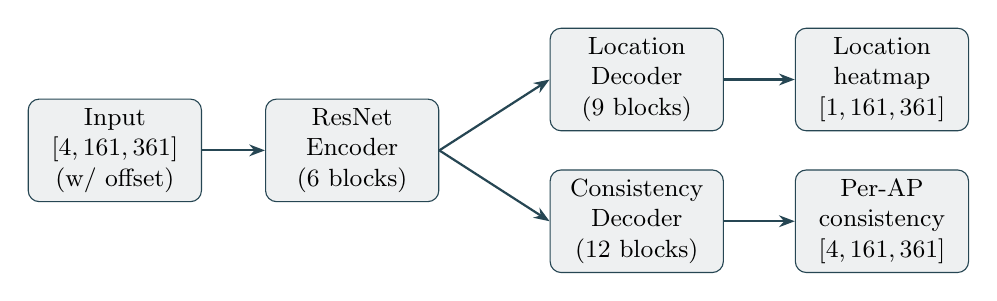
\begin{tikzpicture}[
  box/.style={draw=accent,fill=accent!8,rounded corners,minimum height=1.0cm,
  minimum width=2.2cm,align=center,font=\small},
  arr/.style={-{Stealth[length=2mm]},accent,thick}]
\node[box] (in) {Input\\$[4,161,361]$\\(w/ offset)};
\node[box,right=0.8cm of in] (enc) {ResNet\\Encoder\\(6 blocks)};
\node[box,right=1.4cm of enc,yshift=0.9cm] (dec) {Location\\Decoder\\(9 blocks)};
\node[box,right=1.4cm of enc,yshift=-0.9cm] (off) {Consistency\\Decoder\\(12 blocks)};
\node[box,right=0.9cm of dec] (loc) {Location\\heatmap\\$[1,161,361]$};
\node[box,right=0.9cm of off] (con) {Per-AP\\consistency\\$[4,161,361]$};
\draw[arr] (in) -- (enc);
\draw[arr] (enc.east) -- (dec.west);
\draw[arr] (enc.east) -- (off.west);
\draw[arr] (dec) -- (loc);
\draw[arr] (off) -- (con);
\end{tikzpicture}
\end{center}

The encoder produces a shared latent representation; one decoder predicts the \emph{location}
heatmap and the other enforces \emph{consistency} across APs. At inference only the location
decoder's output is used.

%% ==================================================================
\section{The shared ResNet encoder}

The encoder (\texttt{base\_model = resnet\_encoder}, \texttt{resnet\_blocks = 6}) follows the
standard image-translation generator front-end:
\begin{enumerate}[nosep]
  \item A $7\times7$ input convolution ($4 \to 64$ channels, reflection padding, InstanceNorm,
  ReLU).
  \item Two stride-2 down-sampling convolutions ($64\to128\to256$), halving spatial resolution
  each time.
  \item \textbf{Six residual blocks} at the bottleneck. Each block is
  $\text{Conv}\,3\times3 \to \text{InstanceNorm} \to \text{ReLU} \to \text{Conv}\,3\times3 \to
  \text{InstanceNorm}$, added back to its input.
\end{enumerate}
With $\text{ngf}=64$ base filters, this front-end carries most of the representational capacity.

%% ==================================================================
\section{Decoder 1 --- the Location decoder}

The location decoder (\texttt{resnet\_blocks = 9}) mirrors the encoder: a stack of residual
blocks followed by two \texttt{ConvTranspose2d} up-sampling layers (with
\texttt{output\_padding}\,$=1$) back to $161\times361$, then a $7\times7$ output convolution to a
single channel. Its loss combines a squared term and an absolute term:
\begin{equation}
\mathcal{L}_{\text{loc}} \;=\; \underbrace{\lVert \hat{y}-y\rVert_2^2}_{\text{MSE}}
\;+\; \lambda_{L}\,\underbrace{\lVert \hat{y}-y\rVert_1}_{\text{L1}}, \qquad
\text{(\texttt{loss\_type = L2\_sumL1})}
\end{equation}
where $\hat y$ is the predicted heatmap and $y$ the Gaussian ground truth. The L2 term shapes the
overall heatmap; the L1 term sharpens the peak and suppresses background.

%% ==================================================================
\section{Decoder 2 --- the Consistency (offset) decoder}
\label{sec:consistency}

This is DLoc's defining contribution. Because each AP's input heatmap carries an unknown ToF
offset, the per-AP peaks do \emph{not} coincide. The consistency decoder
(\texttt{resnet\_blocks = 12}, output channels $=4$) is trained to reproduce the
\textbf{offset-free} heatmaps \texttt{features\_wo\_offset} for all four APs simultaneously:
\begin{equation}
\mathcal{L}_{\text{cons}} \;=\; \sum_{i=1}^{N_{\text{AP}}}
\big\lVert \hat{c}_i - c_i^{\text{wo}} \big\rVert_2^2,
\qquad \text{(\texttt{loss\_type = L2\_offset\_loss})}
\end{equation}
By forcing the network to predict heatmaps whose peaks \emph{agree} across APs, it learns to
(i)~remove the ToF offset, (ii)~resolve multipath (pick the direct path), and (iii)~perform
bandwidth super-resolution. The decoder uses all $N_{\text{AP}}$ APs jointly --- a single AP
cannot disambiguate its own offset, but four mutually-consistent APs can.

%% ==================================================================
\section{Three things the consistency decoder learns}

\begin{description}[nosep,leftmargin=1.4cm,style=nextline]
  \item[Offset removal] The input peaks are radially shifted; the output peaks are pulled to the
  true location, made mutually consistent across APs.
  \item[Multipath resolution] When an AP sees two angular maxima (direct + reflected), the
  network selects the direct path by cross-checking against the other APs.
  \item[Super-resolution] Trained with 80\,MHz targets while fed lower-bandwidth (e.g.\ 40\,MHz)
  inputs, the decoder learns to sharpen broad maxima --- recovering resolution the input lacks.
\end{description}

%% ==================================================================
\section{Total objective and training protocol}

The full loss is the sum of the two decoder losses (the encoder itself uses
\texttt{loss\_type = NoLoss}; it is trained through the decoders), with L2 weight regularization:
\begin{equation}
\mathcal{L} \;=\; \mathcal{L}_{\text{loc}} \;+\; \mathcal{L}_{\text{cons}}
\;+\; \lambda_{\text{reg}}\lVert \theta\rVert_2^2 .
\end{equation}

\begin{table}[h]
\centering
\caption{Original DLoc training hyper-parameters.}
\begin{tabular}{@{}ll@{}}
\toprule
Optimizer & Adam ($\beta_1=0.5$) \\
Learning rate & $10^{-5}$ (the paper: \emph{no} rate annealing) \\
Weight decay $\lambda_{\text{reg}}$ & $10^{-5}$ \\
Regularization $\lambda_L$ & $5\times10^{-4}$ \\
Batch size & 32 \\
Normalization & InstanceNorm \\
Init & Xavier ($\text{gain}=0.02$) \\
\bottomrule
\end{tabular}
\end{table}

\paragraph{Inference.} The location is read off as the \textbf{argmax} of the location decoder's
output heatmap, scaled by $0.1$\,m/pixel; the error is the Euclidean distance to the ground-truth
peak. The consistency decoder is used only during training.

%% ==================================================================
\section{Parameter and compute budget}

\begin{table}[h]
\centering
\caption{Size of the original DLoc network.}
\begin{tabular}{@{}lrr@{}}
\toprule
Component & Resnet blocks & Role \\
\midrule
ResNet encoder        & 6  & shared feature extractor \\
Location decoder      & 9  & predicts location heatmap \\
Consistency decoder   & 12 & enforces multi-AP agreement \\
\midrule
\textbf{Total}        &    & $\approx 16.5$\,M parameters, $\sim$81\,GFLOPs, $\sim$66\,MB weights \\
\bottomrule
\end{tabular}
\end{table}

This heavy footprint --- three ResNet stacks at 64 base filters --- is precisely what motivates
the lightweight redesign documented in \texttt{03\_model\_architectures}. The next document
(\texttt{02\_dataset}) describes the data on which all of this is trained and evaluated.

\end{document}
